\section{Detalizuotas vertės grandinės modelis}
BPMN modelyje galima pastebėti įmonės valdymo veiklų supratimo neapibrėžtumus \cite{bpmnPorterModel}. Taip yra todėl, kad išorinio modeliavimo metodai neparodo informacijos arba resursų transformavimo priežasčių. Tačiau įmonę galima analizuoti ir transakcinių darbų sekų modelio (\ref{img:pdca} pav) požiūriu.  
\begin{figure}[H]
	\centering
	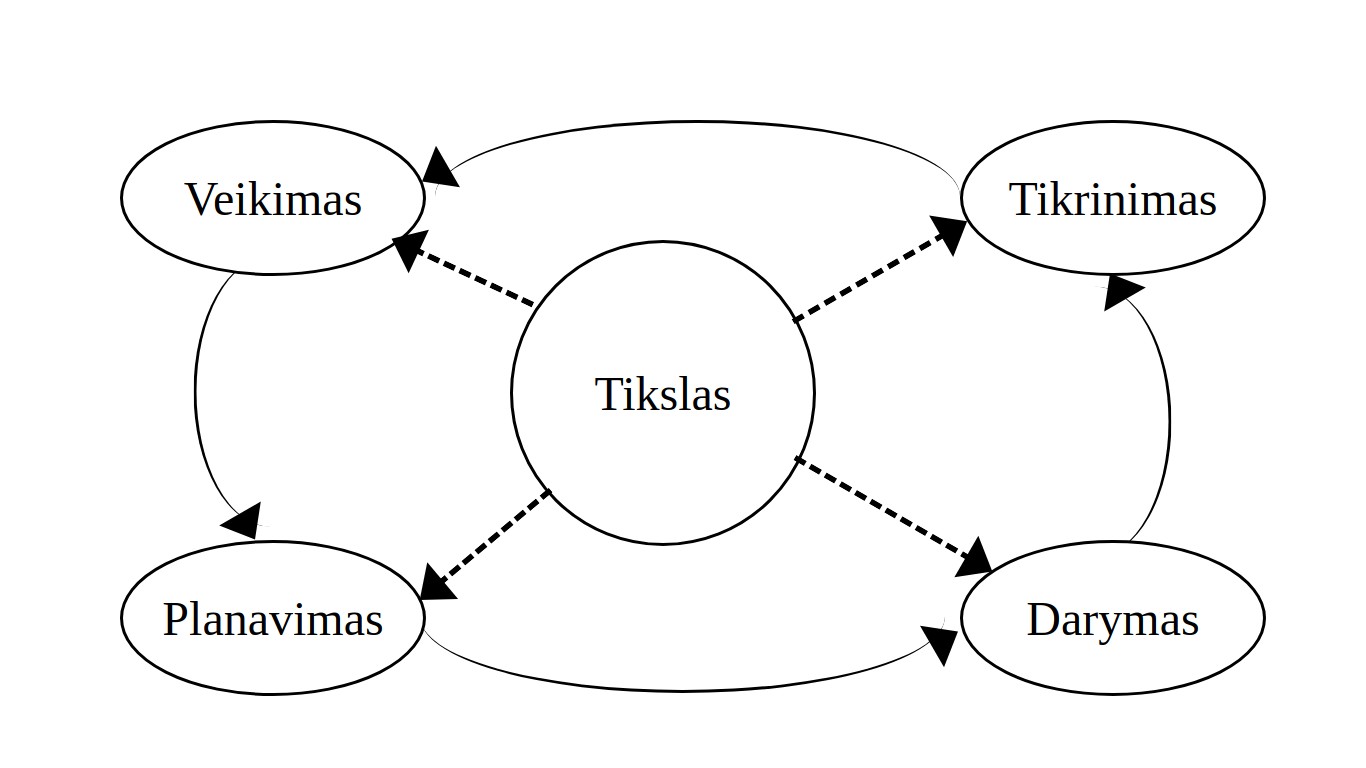
\includegraphics[width=10cm]{img/pdca}
	\caption{Transakcinių darbų sekų modelio pavyzdys}
	\label{img:pdca}
\end{figure} 

Darbe įmonės procesas bus nagrinėjamas kaip transakcijų visuma. Materialios veiklos atskiriamos nuo valdymo veiklų. $P_i$ žymi veiklos procesą, kuris transformuoja žaliavas, medžiagas, energiją ir formuoja materialią išeigą. $F_j$ yra veiklos valdymo funkcija, informacijos (duomenų, žinių) transformavimo veikla, būtina valdant procesą $P_i$. Modelis yra suskirstytas į valdymo transakcijas $ MT_{ij} = F_j \times P_i$. Tokiu būdu pateikiama daugiau informacijos apie įmonę. Diagrama bus vaizduojama kaip detalizuotas M. Porterio vertės grandinės modelis (\ref{img:detalized_porter_vcm} pav).

%TODO: show goles in diagram
\begin{figure}[H]
	\centering
	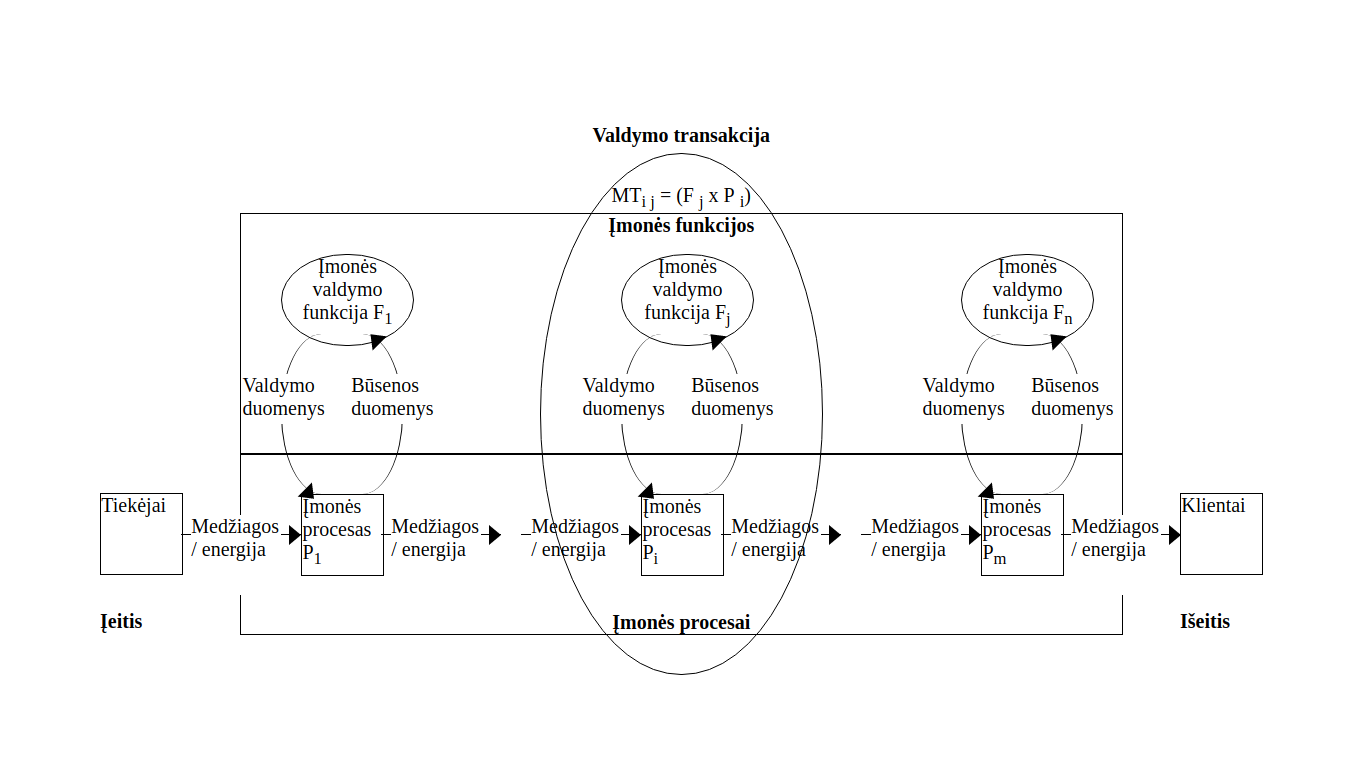
\includegraphics[height=8cm]{img/detalized_porter_vcm}
	\caption{Detalizuotas M. Porterio vertės grandinės modelis}
	\label{img:detalized_porter_vcm}
\end{figure} 

Valdymo funkcija $F_j$ gali būti suskaidyta smulkiau. (\ref{img:splitted_management_function} pav) parodytas pavyzdys kai $F_j$ susideda iš smulkesnių dalių $F_{j1}$, $F_{j2}$ ir $F_{j3}$. Kartu visa tai suteikia veiklos procesui $P_i$ valdymo duomenis kuriuos jis panaudoja vykdymui. Vėliau grąžinami būsenos duomenys, jie panaudojami valdymo funkcijoje ir ciklas kartojasi.

\begin{figure}[H]
	\centering
	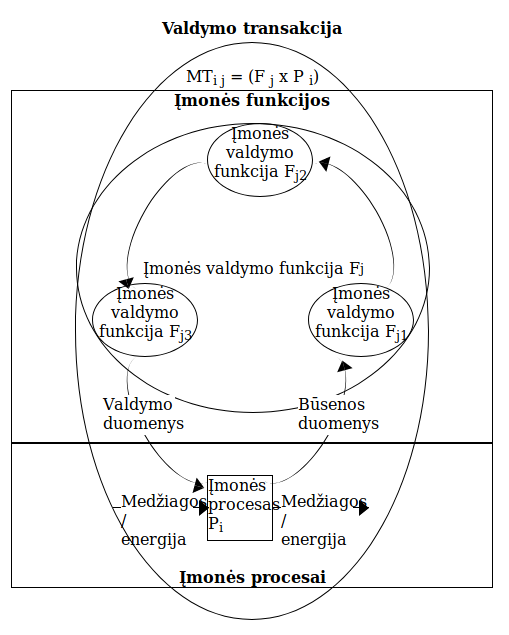
\includegraphics[width=7cm]{img/splitted_management_function}
	\caption{Valdymo funkcijos $F_j$ išskaidymo pavyzdys}
	\label{img:splitted_management_function}
\end{figure} 
